% LaTeX introduction practical 2/2

% Dr. Noel Juvigny-Khenafou
% University of Koblenz-Landau, Winter semester 2020

% In this practical we will create a rough template for a scientific manuscript to go around some of the features of LaTeX.
% You will find the necessary picture files directly on the GitHub.
% You can then later use this template and improve it for your own manuscript writing.
% Enjoy !

\documentclass[11pt, a4paper]{article}


\title{My introduction to LaTeX}
% this package enables us to create affiliations for the authors
\usepackage{authblk}
\author[1]{John}
\author[2]{Mike}
\affil[1]{Department 1, University 1}
\affil[2]{Department 2, University 2}

\date{Date of submission (or last edit)}

\usepackage[utf8]{inputenc} % enables to enter accent for Mac and Linux users
% \usepackage[latin1]{inputenc} on Windows

\usepackage[english]{babel}
\usepackage{helvet}
\usepackage{microtype}
\usepackage {graphicx}
\graphicspath{ {images/} } % define the path of where the images are stored

% let's add some new package for extra features

% we can first customise the margins with the geometry package
\usepackage[a4paper, inner=1.7cm, outer=2.7cm, top=2cm, bottom=2cm, bindingoffset=1.2cm]{geometry}

% package to compact lists
\usepackage{enumitem}

% package to make index
\usepackage{index}
\makeindex

% package to make beautiful math equations
\usepackage{amsmath}

% package used to easily move pictures around
\usepackage[export]{adjustbox}

%package to customise captions
\usepackage{caption}

% package to add multiple figures together and have subcaptions
\usepackage{subcaption}

% this package is to indent the first line of a paragraph following a section. By default LaTeX does not indent the first line after a section.
\usepackage{indentfirst}

% this package cancels the indent created when you open a new paragraph.
% \usepackage{parskip}

% set the spacing between paragraph
\setlength{\parskip}{1em}

% set the spacing between lines
\renewcommand{\baselinestretch}{1}

% package Biblatex to manage bibliography
%\usepackage[backend=bibtex, style=authoryear, sorting=nyt]{biblatex} % the style of the reference can be easily adjusted using the optional arguments. Note that an other common backend with biblatex is biber. but you need to use pdflatexmk
%\addbibresource{/Users/Noel/Documents/latex/library.bib} % this line is to give the path of the database

% package to cite using bibtex instead of biblatex
\usepackage{cite}
\usepackage{besjournals}

% all the packages are loaded and adjustment made in the preamble.
% we now start our document.

\begin{document} 
\maketitle  % we now create the title page of our manuscript.
\pagenumbering{arabic} % we can add the page number to make it easier to refer to the right place when editing.
\setcounter{page}{1} % we can chose when we want to start numbering our pages.
\thispagestyle{empty} % and we can choose to keep or remove the page numbering for individual pages.
\pagebreak % and we create a new page for our abstract and keywords.

\begin{abstract}
We have now created our first little LaTeX document.
\end{abstract}
\par % this is an other way to start a new paragraph 
\textbf{\underline{\textit{Keywords:}}} keyword 1, keyword 2, keyword 3 % see how you can modify the appearance of words in the text
% by nesting command line.
\pagebreak 

\tableofcontents % add a table of content based on our indexing

%we can then now separate our document between the different sections needed
% to include chapter with \chapter{your chapter's name} the document class must be set as book

\pagebreak

\section{Introduction} % by using section{} we can automatically make numbered sections throughout the document.

Type the text that you want to have in your introduction here. Let's make this paragraph a little longer so you can see the start of the new paragraph better. % now, press "enter" twice to insert a blank line and start a new paragraph. 


You can see here that when a double break is inserted we open a new paragraph. % see the indent to see the start of the new paragraph
But sometime we also want to just start a new line without the new paragraph.\\ % the double backslash starts a new line.
Like this. 
\par
Sometimes we want to include our hypotheses as a bulleted list:

\begin{itemize}
	\item Hypothesis statement 1
	\item Hypothesis statement 2
\end{itemize}

Or as a numbered list:
\begin{enumerate}
  \item Hypothesis statement 1
  \item Hypothesis statement 2
\end{enumerate}

\section{Material and methods}
\subsection{Location}
\subsection{Sampling}
\subsection{Data analysis}

When we explain how we handle the data we sometime want to add some mathematical equations. Mathematical equation can be added \textit{in-line}, \begin{math}E=mc^2\end{math}, or in \textit{display}:
\begin{equation} % for the equation to be unumbered use \begin{equation*}
E=mc^2
\end{equation}
% note that there are other ways to add equations into a LaTeX documents and its up to you which one you feel more comfortable with
But we also have situations where we have successive equations to display:
\begin{align*} % notice how the numbering was removed using the *
f(x) = x^2+3x+2\\ 
f(x) = x^2+3x+2 
\end{align*}

\section{Results}

In this section let's see how to include some graphs \& tables as you would in a results section.\\ 
% you can see here that to add special character it is needed to use a "\". To introduce a backslash though it is slightly different
% and you need to write \textbackslash
Example to insert a backslash: \textbackslash\\ % note that the double backslash introduces a new line but not a new paragraph.
% Be very careful between the two.
You can find a list of how to insert the other characters easily on Internet.

%now you can see here that if I have only on break after a dot, in the printed document the break is ignore and we remain in the same paragraph
% we now insert an image
% define where we want the image place
% h: Here, t: Top of the page, b: Bottom, p: Separate page, !: improves the float
We now insert a picture: % we can see here that the double slash insert a line spacing.
\begin{figure}[ht!]
\centering
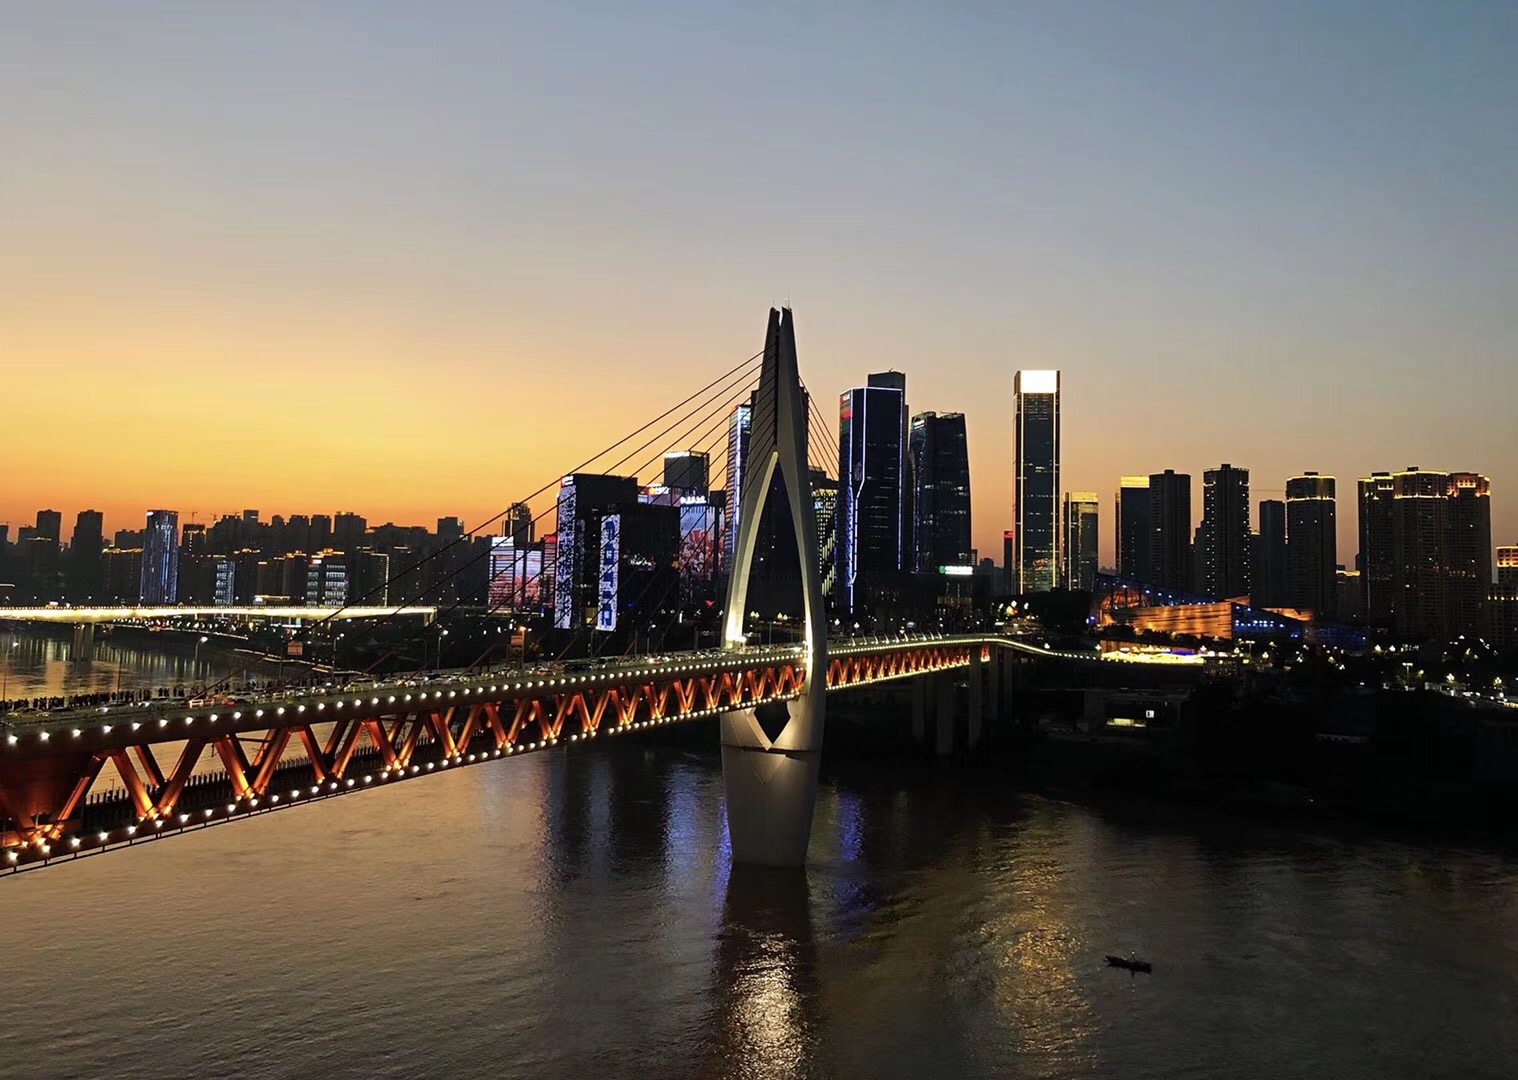
\includegraphics[width=8cm]{chongqing2019.jpg} % there is no need to adjust the height as this is done automatically.
\end{figure}
\newpage % sometimes you need to move some text or content to the next page for clarity. Try to remove that line and see what happens.

And we can add a caption:
\begin{figure}[ht!]
\centering
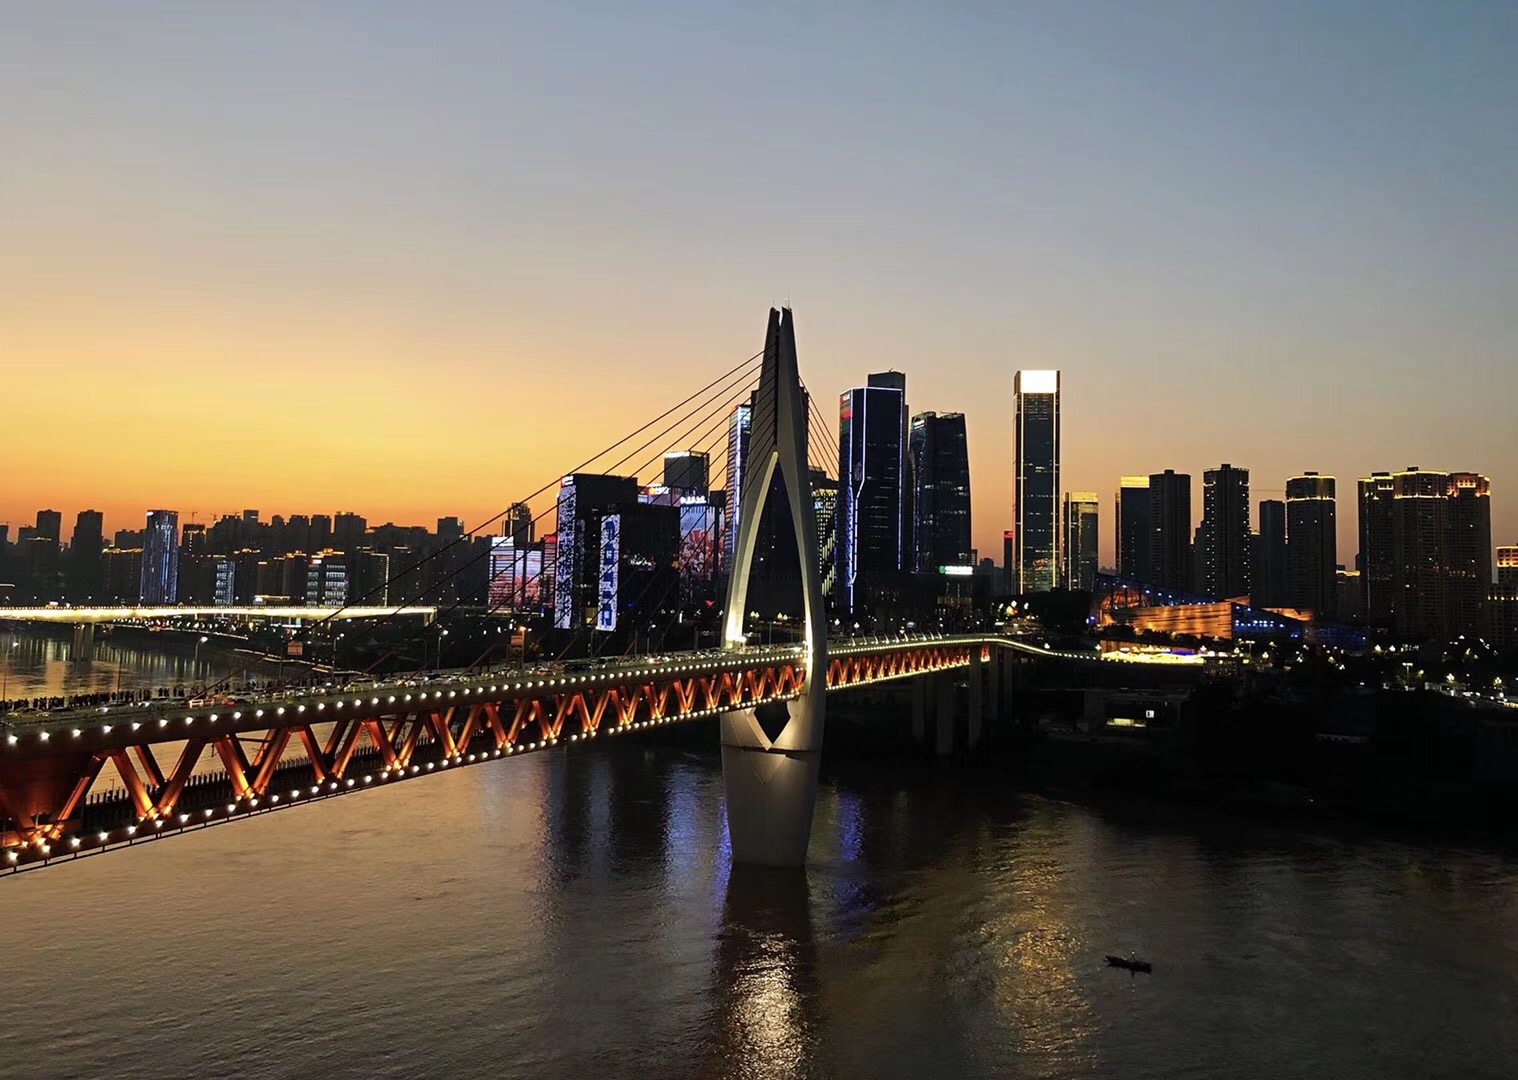
\includegraphics[width=8cm]{chongqing2019.jpg} 
\caption{Chongqing 2019. $\copyright$\textit{Juvigny-Khenafou}}
\label{picture1} % it is sometimes interesting to also add a label to the figure that way it can be easily referred to at later staged when writing.
\end{figure}

We can also play with the positioning of the figure:
% to the left
\begin{figure}[ht!]
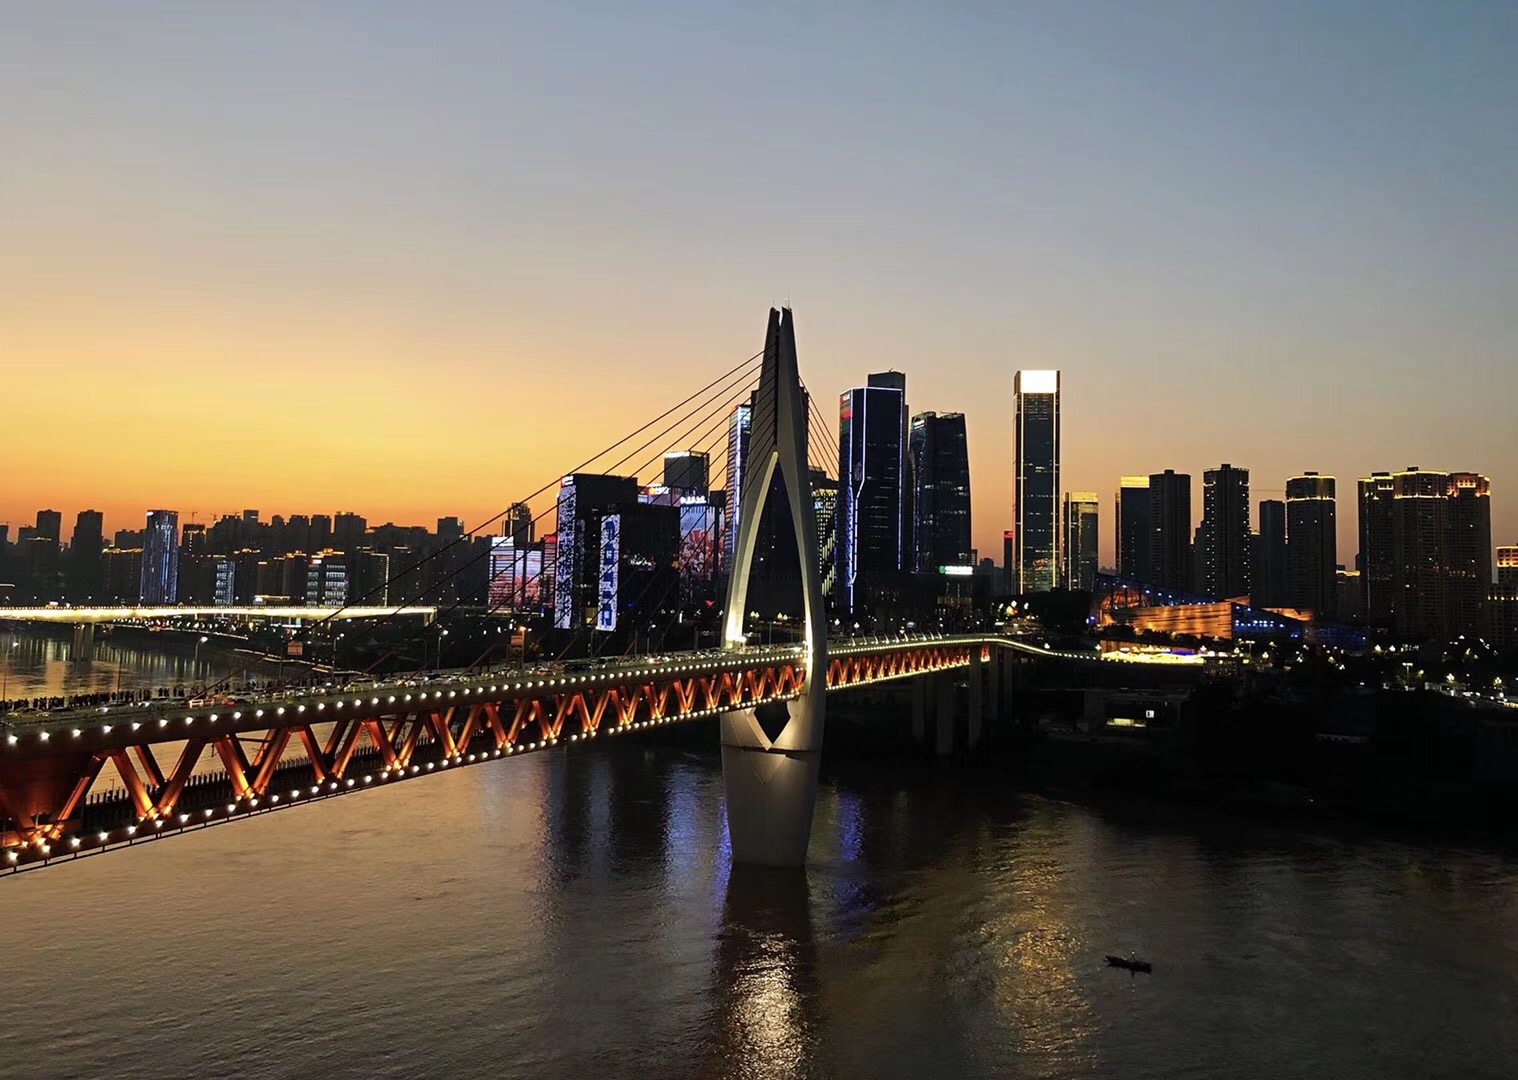
\includegraphics[width=8cm]{chongqing2019.jpg} % notice how the \centering is removed here to assume the default positioning
\captionsetup{justification=raggedright, singlelinecheck = false} % we can use the \captionsetup command within an environemnent to modify specific caption without affecting the other figures.
\caption{Chongqing 2019. $\copyright$\textit{Juvigny-Khenafou}}
\label{picture2}
\end{figure}
\par

% to the right
\begin{figure}[ht!]
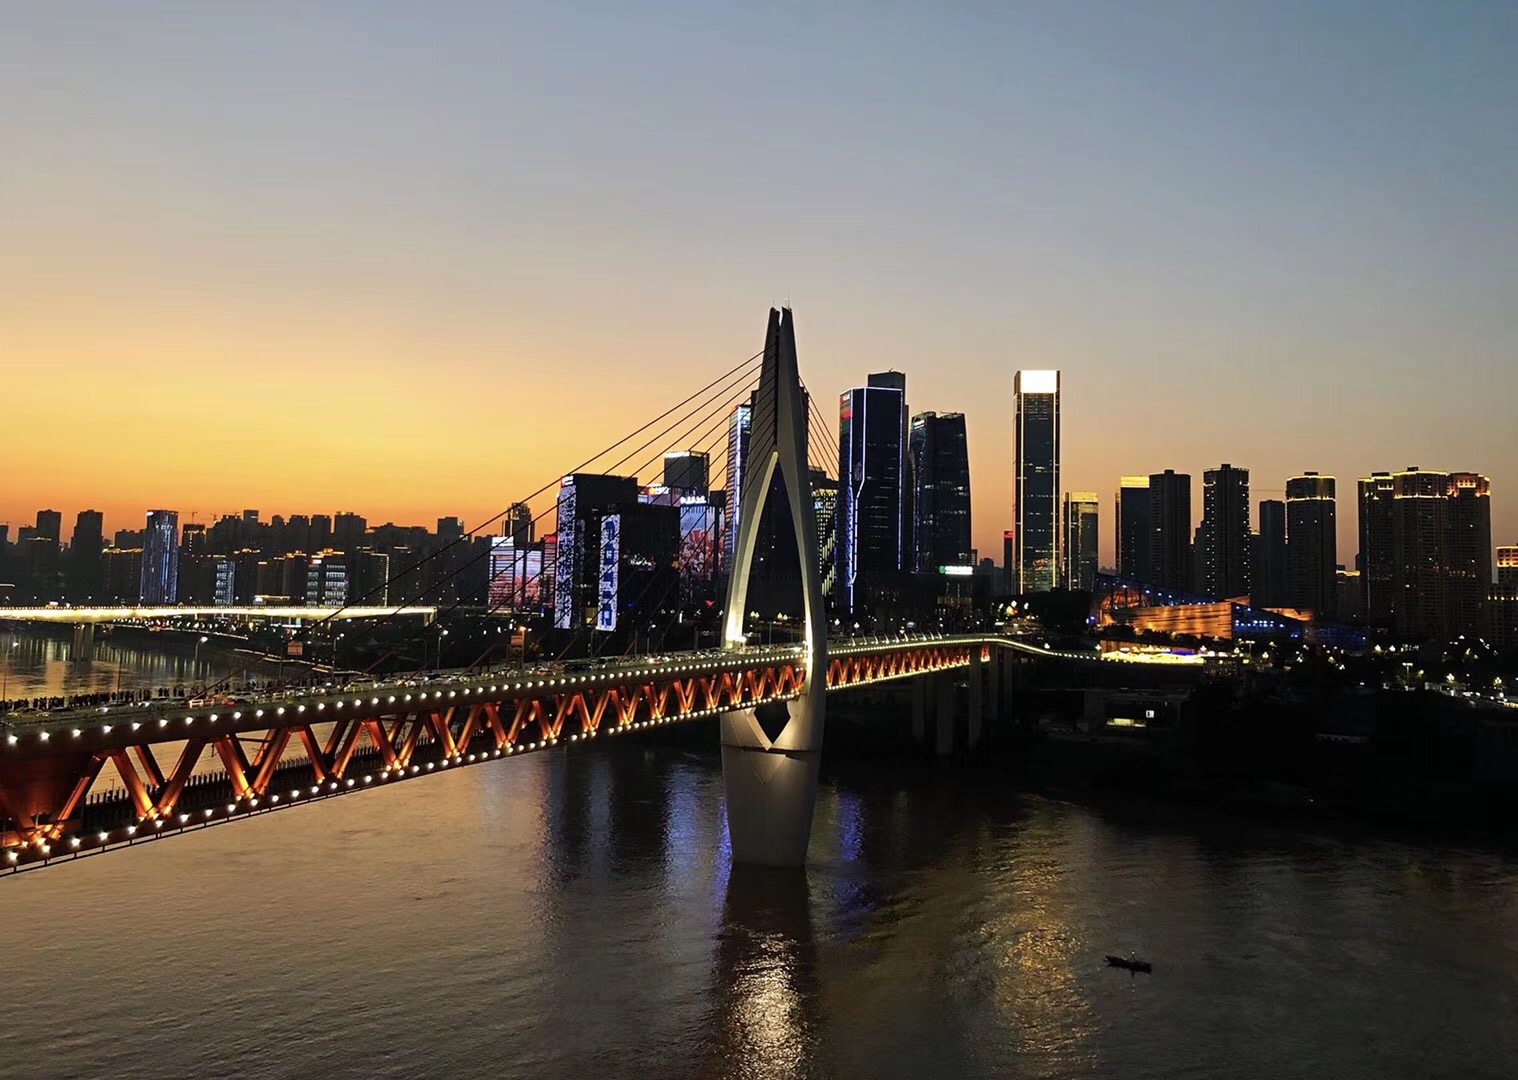
\includegraphics[width=8cm, right]{chongqing2019.jpg} % notice how the centering is removed here to assume the default positioning
\captionsetup{justification=raggedleft, singlelinecheck = false} 
\caption{Chongqing 2019. $\copyright$\textit{Juvigny-Khenafou}}
\label{picture3} 
\end{figure}
\newpage
\par

Or we can add multiple pictures together:
\begin{figure}[ht!]


	\begin{subfigure}{0.5\textwidth}
	\centering
	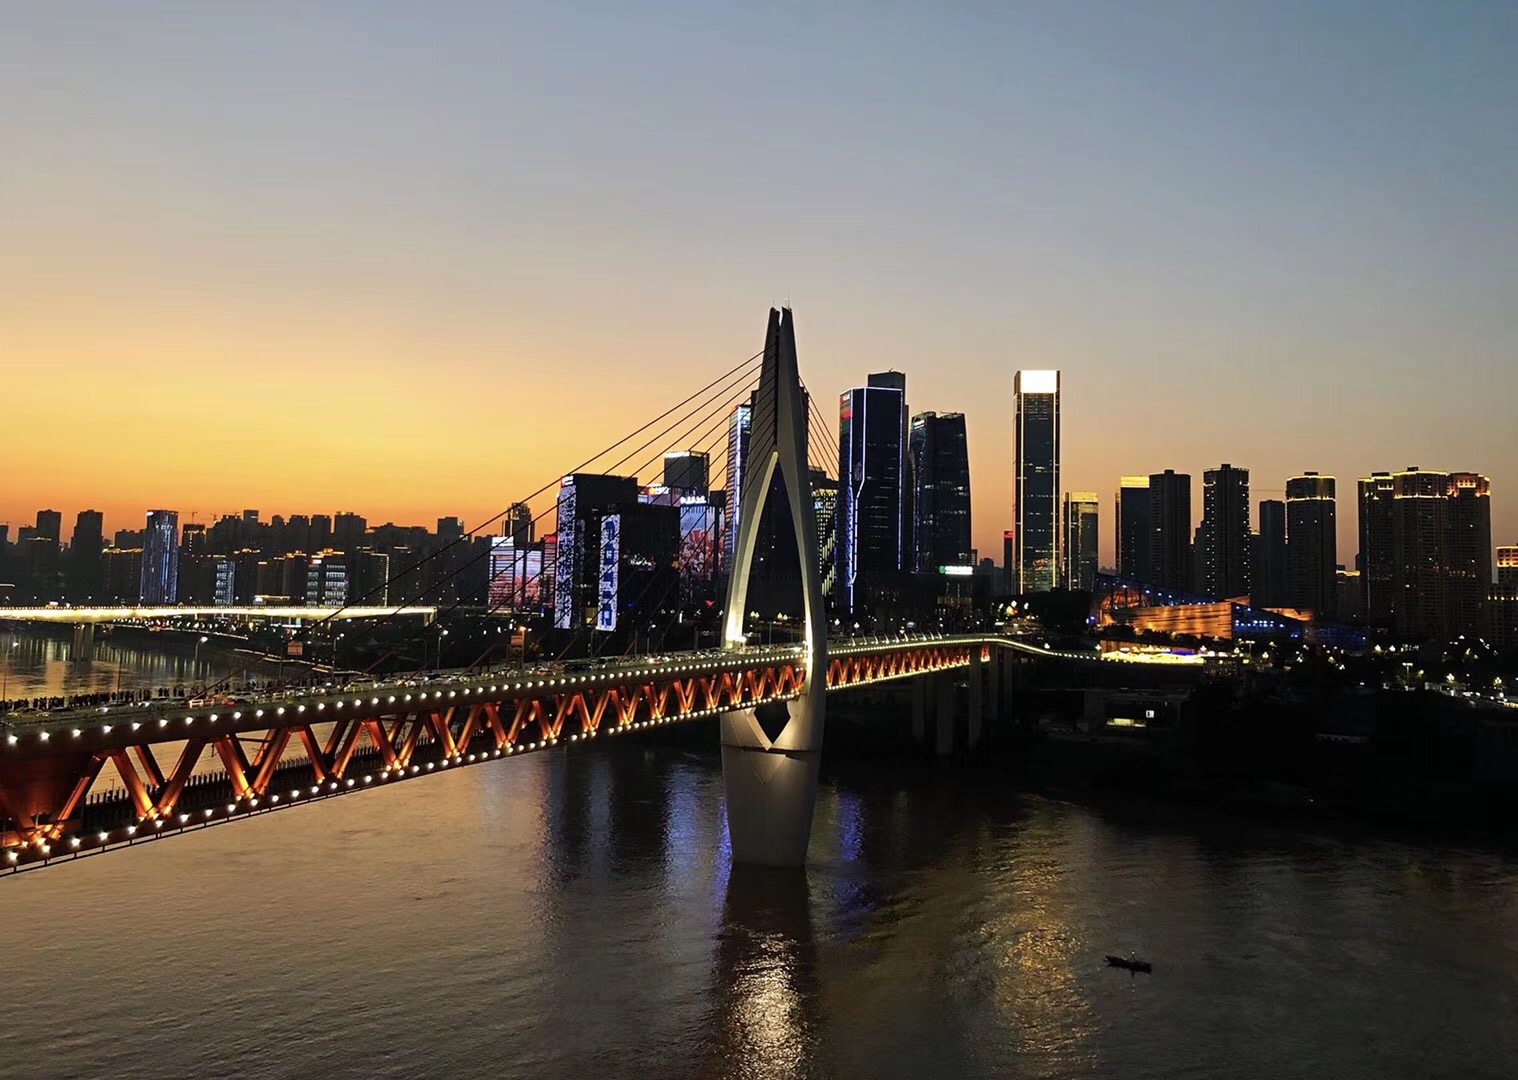
\includegraphics[width=0.9\linewidth, height=5cm]{chongqing2019.jpg} 
	\caption{Chongqing 2019}
	\label{fig:subim1}
	\end{subfigure}
	\begin{subfigure}{0.5\textwidth}
	\centering
	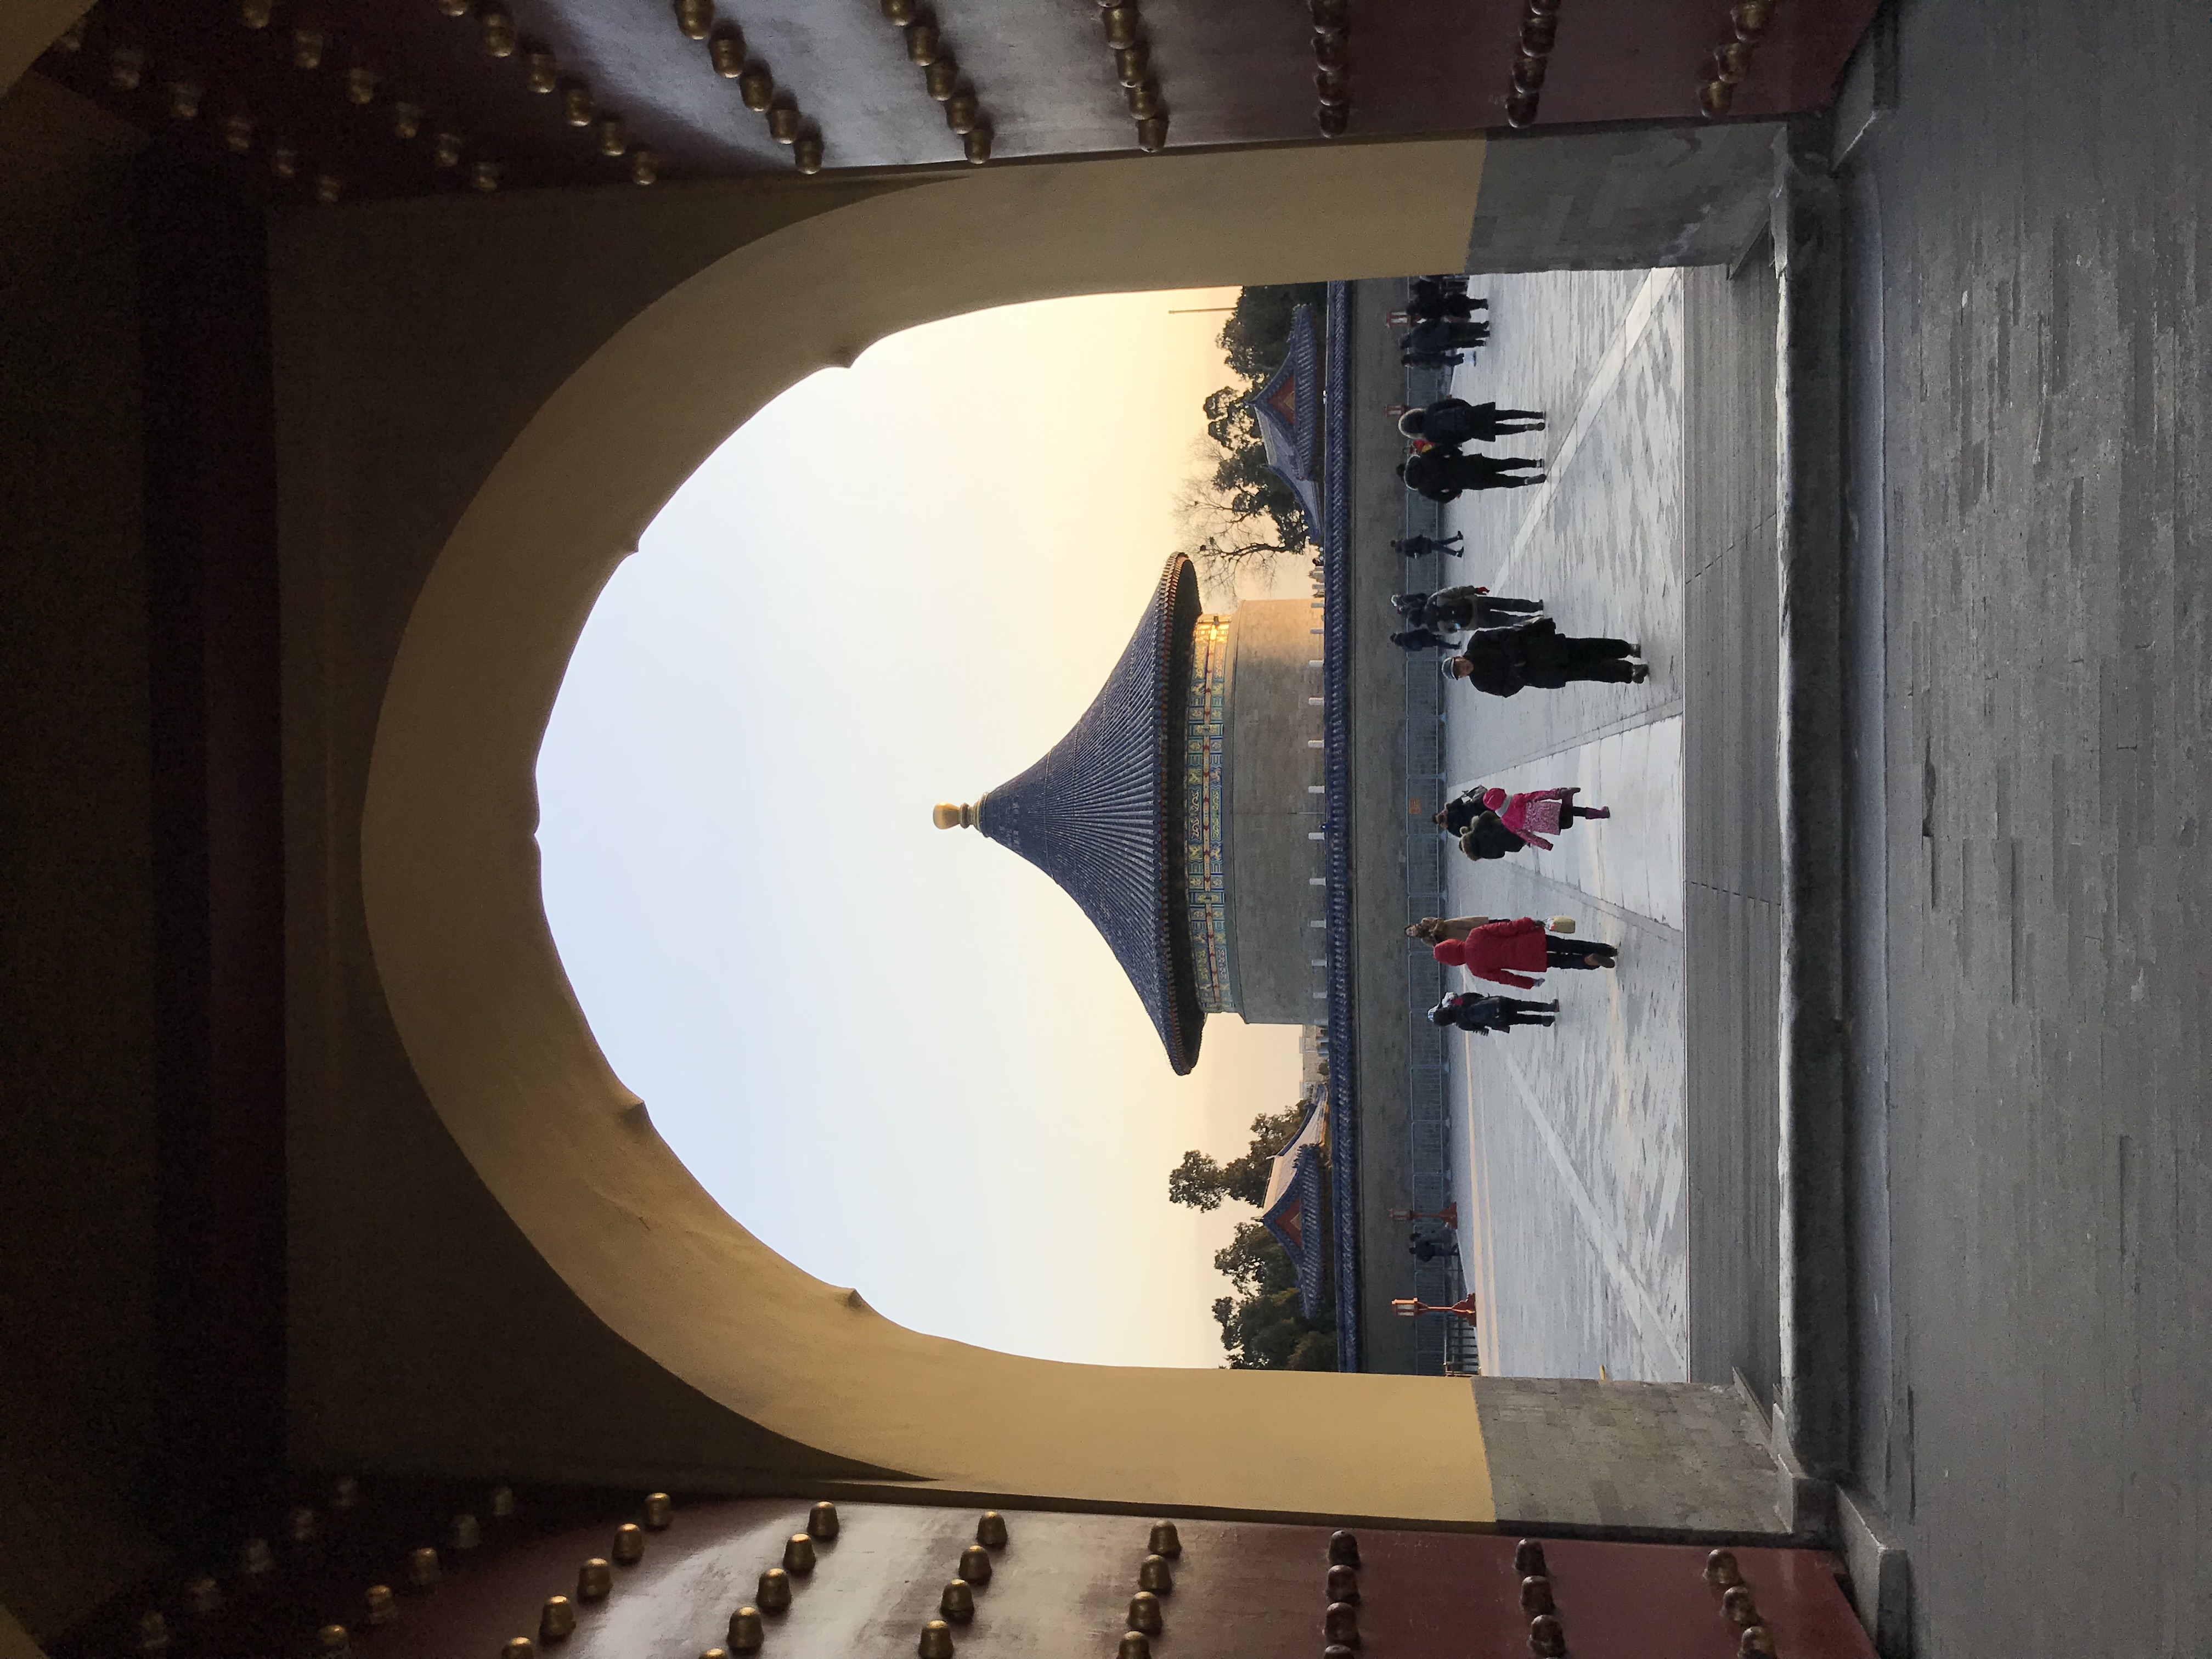
\includegraphics[width=0.9\linewidth, height=5cm, angle=270]{beijing2018.jpg}
	\caption{Beijing 2018}
	\label{fig:subim2}
	\end{subfigure}

\caption{Chongqing \& Beijing $\copyright$\textit{Juvigny-Khenafou}}
\label{picture4}
\end{figure}
\par

Tables also come as an handy way to summarise key findings:
\begin{table}[ht!]
\centering
\caption{table caption}
\begin{tabular}{c | c c} % see that the | character introduces a vertical line
cell1 & cell2 & cell3 \\ 
\hline % and this line introduces a horizontal line
 cell4 & cell5 & cell6 \\  
 cell7 & cell8 & cell9    
\end{tabular}
\label{table:1}
\end{table}


\section{Discussion}
The final point that we want to touch in this practical is the referencing. Before you can do any referencing you need to create a bibtex library with your references. To do that you can use your reference manager software (Mendeley in my case) and create a synchronized library at the root of your LaTeX folder. Then you'll be able to call in references directly in all your subsequent LaTeX documents.
\par

%For instance Lawton had a lot to say about what species do in an ecosystem \parencite[manually add front elements,][manually add end elements]{Lawton1994}. % note that this time instead of using Latex typesetting we use "pdflatexmk" this allow the compiling of all the files in a single run. Otherwise you need 4 runs to compile the different files (latex -> bibtex -> latex -> latex)
\par
%There are also time when we want to cite \textcite{Lawton1994} directly in the text.


\addcontentsline{toc}{section}{Acknowledgements} % this command line enables to add unnumbered sections to the table of content
\section*{Acknowledgements}

\addcontentsline{toc}{section}{Funding}
\section*{Funding}

\addcontentsline{toc}{section}{References}
%\printbibliography

\newpage %add a page break and don't stretch the text to fill the previous one.

\addcontentsline{toc}{section}{Appendices}
\section*{Appendices}

We can also cite using bibtex instead of biblatex. For example: \cite{Lawton1994}. 
\par

\bibliography{/Users/Noel/Documents/latex/library}{}
\bibliographystyle{besjournals}



\end{document} 






